\newcommand{\Thesiscolor}{tud1b}
\newcommand{\Thesiscolorbright}{tud1a}
\documentclass[
type=bsc,			% Bachelor Thesis
accentcolor=\Thesiscolor,	% Blau
colorbacktitle,		% Farbige Titelseite
11pt				% Schriftgröße
]{tudthesis}

\usepackage[utf8]{inputenc} % Kodierung
\usepackage[english]{babel}	% Sprache

% Grafiken
\usepackage{graphicx}
\usepackage{subcaption}
\usepackage{tikz}
\usepackage{tikz-3dplot}
\usetikzlibrary{arrows.meta}
\usepackage[skins]{tcolorbox}	% for putting images into rectangles

% Tabellen
\usepackage{booktabs}

% Mathe
%\usepackage{bm}
\usepackage{amsmath}
\usepackage{mathtools}

% Algorithmen
%\usepackage[]{algorithm2e}

\usepackage{blindtext}		% Dummytexte

\usepackage{cite}			% Bibliography

\usepackage{hyperref} 		% should be loaded as last package, adds links to table of contents

% Referenzen
%\usepackage{cleverref}
\graphicspath{{img/}}

% custom todo
\newcommand{\todo}[1]{\textcolor{red}{\large \emph{\bfseries{TODO:}}} #1 \\}

% Bold vectors
\let\vecarrow\vec 					% save old vector definition
\renewcommand\vec[1]{{\mathbf{#1}}}

% shortcuts
\newcommand{\etal}{\textit{et al}.\ }
\newcommand{\ie}{\textit{i}.\textit{e}.\ }
\newcommand{\eg}{\textit{e}.\textit{g}.\ }
\newcommand{\Eg}{\textit{E}.\textit{g}.\ }

% images size
\newcommand{\imgsize}{192}
\newcommand{\facesize}{64}

% shortcuts for often used mathematical terms
\newcommand{\distr}{\mathbb{P}_d}
\newcommand{\distt}{\mathbb{P}_\theta}
\newcommand{\genInputZ}{z}
\newcommand{\genInputB}{y}
\newcommand{\genWithZInput}{G(\genInputZ)}
\newcommand{\genWithInput}{G(\genInputZ, \genInputB)}
\newcommand{\discInput}{x}
\newcommand{\discWithInput}{D(\discInput)}

% figure sizes
\newcommand{\threeFigOnePageSize}{7.18cm}

% KL doppelstrich
\DeclarePairedDelimiterX{\infdivx}[2]{(}{)}{%
	#1\;\delimsize\|\;#2%
}


\thesistitle{Unconstrained Shape from Shading using CNN}{}

\author{Daniel José Ceballos Jung}
\birthplace{Stuttgart}

\referee{Stefan Roth, Ph.D.}{Stephan Richter, M.Sc.}{}

\department{Fachbereich Informatik}
\group{Visual Inference}
\setinstitutionlogo{images/logos/vi-logo.png}

\includeonly{
%	chapters/abstract,
%	chapters/introduction,
%	chapters/related-work,
	chapters/background,
%	chapters/dataset,
%	chapters/model,
%	chapters/experiments,
%	chapters/conclusion,
}

\begin{document}
	% --- Title page --- %
	\makethesistitle
	
	\affidavit[23.07.2018]{Daniel Ceballos}
	
	\section*{Acknowledgements}
	First of all, I want to thank Professor Stefan Roth for giving me the opportunity to write my thesis in his visual inference group.\\ \\
	Further, I thank my supervisor Stephan for being a great help, giving lots of input and guiding me through this thesis. \\ \\
	I would like to thank my friend Janne for investing a lot of time in proofreading and giving great input on writing. \\ \\
	Eventually, I thank my family for their trust and unconditional support.
	\clearpage
	
	\begin{abstract}
		\include{chapters/abstract}
	\end{abstract}
	
	% --- Table of contents --- %
	\tableofcontents
	
	% --- Main Document --- %
	\chapter{Introduction}
	Computer vision is the development of models and algorithms, to interpret digital images and to get a better understanding of the visual world. One aspect of understanding the world is the recovery of shapes. The goal of shape recovery is to obtain three dimensional informations about a scene or an object from one or more 2D images. The estimated shape can be represented in various ways. 
	\\
	One way to represent the shape of an object is using depth $Z(x,y)$. Therefor either the relative surface height above the x-y plane ore the relative distance from surface to camera is measured. The depth map encode near points on the surface darker and distant point lighter to a gray scale image. 
	\\
	Another way to express the shape of an object is to use surface normal $(n_x, n_y, n_z)$. The surface normal is the direction of a vector perpendicular to the tangent plane of the surface point and can be calculated by taking the cross product $l \times s$ of two vectors that span the plane, e.g. between the vector of incident ray $l$ and the orientation vector of the camera $s$. To obtain depth informations, the surface gradient $(p,g) = (\frac{\partial z}{\partial x}, \frac{\partial z}{\partial y}) $ is used, since it indicates the rate of the depth change along the $x$- and $y$-axis. For visualization the normal map then encode the direction of the vectors to the RGB colors.
	%TODO Figure normal map (koordinaten system) depth bsp 
	\\ 
	\\
	Shape recovery is a classic and hard to solve problem in computer vision. Therefore several methods and techniques have been developed~\cite{Horn_SHAPE_FROM_SHADING_1970, Shape_from_X_psychophysics_and_computation}. In computer vision techniques to recover the shape of an object are called shape-from-X, where X can stand for: focus, motion, shading, stereo, texture, etc. In this thesis the shape-from-shading technique will be used to recover an objects shape. Shape-from-shading uses the shading of an object's surface to recover informations about the 3D shape of this object. Artists early learned the principle of using lighting and shading to create the illusion of depth in there paintings. To solve shape-from-shading it is important to a
	%TODO beschreiben warum shape from shading schwer ist
	\\
	\\
	%TODO Problem Bild verarbeitung vortschritt in neuronalen Netzen usw.
	Humans solve problems like shape recovery (shape-from-shading) with ease. However they are very hard to solve for a computer.	
	\\ 
	\\	
	MarrNet~\cite{MarrNet} is an two step end to end trainable model that uses an encoder-decoder convolutional neuronal network architecture in addition to reconstruct the three-dimensional shape of an object using 2.5D sketches. Therefor the first step of the Model predicts the depth map, surface normals and silhouette of an object given a single RGB image. However like the most shape-from-shading techniques MarrNet assume orthographic images, which are not very realistic. 
	\\
	The hypotheses of this theses is that with increasing perspective distortion the accuracy decreases. Therefore a large scale dataset (chapter \ref{sec:dataset}), containing four types of image projections, were created, trained and evaluated (chapter \ref{sec:exp}) on the MarrNet model.
	% \begin{figure}
	%	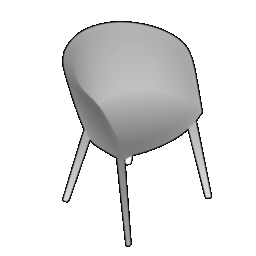
\includegraphics[height=0.1\textheight]{introduction_depth.png}
	%	\caption{A boat.}
	%	\label{fig:boat1}
	% \end{figure}

	\chapter{Related Work}
	In computer vision shape-from-shading is an long standing and well studied problem. And has therefore an extensive literature~\cite{Shape_from_shading_A_survey, Perceiving_Shape_from_Shading}. Besides the classical numerical approaches~\cite{Numerical_methods_for_shape_from_shading}, machine learning solutions~\cite{Training_many_parameter_shape_from_shading_models, A_neural_network_approach_for_shape_from_shading} become more and more relevant. However recent advances in Convolutional Neuronal Networks~\cite{ImageNet_Deep_Convolutional_Neural_Networks} have hardly been implemented yet to the shape from shading problem due to te lack of suitable training data.
	
\section{Classic Shape-From-Shading}
\label{sec:relwork:SFS}

	% Geschichte von Shape from shading
	Shape-from-shading is a long standing problem in computer vision. It uses the shading of an object's surface to obtain information about it's three-dimensional shape. The first shape-from-shading technology was developed by Horn et al.~\cite{Horn_SHAPE_FROM_SHADING_1970}+ in the early 1970s. He showed, that for many surfaces the fraction of the incident light which is reflected in a certain direction is a smooth function. If the surface reflection function and the position of the light source is know, the shape can be obtained from the shading. Due to the fact that the equations are quite complex Horn suggested to simplifies the conditions of the method. One proposed simplification is to assume a single withe point light source and Lambertian reflectance. Under this assumptions Lambertian shape-from-shading was explored for decades. However the constraints given by the illumination are not sufficient to specify the local orientation. To restrict shape estimation chromatic illumination~\cite{Shape_from_shading_under_complex_natural_illumination, Shape_estimation_in_natural_illumination} is used. It not only restrict the shape estimation significantly but also it approximates real-world environments a lot better. However, since both methods strongly depend on favorable known illumination, they are not suitable for practical applications. Apart from that it is important to be aware that  some impossible shaded images exist, witch could not been arisen from shading on a smooth surface with uniform reflecting properties and lightning~\cite{Impossible_shaded_images}. For those images shape-from-shading will not give the correct solution.
	\\ \\
	Instead of assuming a point light source, estimating the shape based on the material properties of an object is a promising approach. So if the orientation clues in the lighting environment are exploited, one can determine the objects shape along with the objects bidirectional reflectance distribution function (BRDF)~\cite{BRDF_Shape_and_reflectance_from_natural_illumination}. Nonetheless a high quality environment map is necessary as this method exploits the contextual information embedded in the lightning. Also shape-from-shading using the objects BRDF requires a known illumination. It has been shown, that natural images have simple statistics~\cite{Statistics_of_Natural_Image_Wood, Relations_between_the_statistics_of_natural_images}. Given this fact natural image statistics can be used to eliminate the constrain of a known illumination and albedo and to estimate the shape of an object as part of a decomposition of a single image into its intrinsic components~\cite{Shape_albedo_and_illumination_from_a_single_image}. Therefore a generative model have to be optimized. Making the extension of the model with new cues very complex. 


\section{Machine Learning}
\label{sec:relwork:ML}	
	
- versiedene ML ansätze zu SFS und deren einschränkungen


	%Überleitung zu CNN virher marrnet und den anderen CNN ansatz erklären
	Despite this methods recent advances of Convolutional neural networks have hardly been implemented and studied yet. 
	
\subsection{Convolutional Neural Networks}
	In 2012 Hinton et al.~\cite{ImageNet_Deep_Convolutional_Neural_Networks}
\label{sec:relwork:CNN}
- was sind CNN? \\
- neuste fortschritte  \\
- hier schon ResNet erklären? 
	

	\chapter{Background}
	In this chapter a brief intruduction is given about the basic techniques used in this thesis.
	Section \ref{sec:background:SFS} gives a short description of the classic shape-from-shading problem and the basic assumptions. In section \ref{sec:background:CNN} a short introduction on convolutional neuronal networks  is given and how to make training deep neuronal network architectures more easy \ref{sec:background:mlCNN:resnet}.
	
%#########################################################
\section{Shape recovery using shading}
\label{sec:background:SFS}
	Three components are essential to the shape-from-shading (SFS) problem. The object whose shape should be estimated, the light source and the camera which produces the image of the surface  (see figure \ref{fig:surface_normal}). Considering a three-dimensional coordinate system $O(x,y,z)$ attached to the camera and $O(z)$  attached to the to the optical-axis then $O(x,y)$ coincides with the image plane:
	
	\begin{equation}
		\vec{x} = f \frac{x}{z}
		\quad \quad \quad  \quad 
		\vec{y} = f \frac{y}{z}
	\end{equation}
	
	where $(\vec{x},\vec{y})$ are the image coordinates of a point $(x,y,z)$ made by a camera with focal length $f$. 	
	As the image irradiance and the object irradiance are proportional, the shape-from-shading problem can then be formalized as the "image irradiance equation":
	
	\begin{equation}
	\label{eq:img_irradiance}
	R(p,q) = E(x,y)
	\end{equation}
	
	where $E(x,y)$ is the grayscale level (irradiance) of the image in point $(\vec{x},\vec{y})$ and $R(p,q)$ is the reflection function, giving the amount of re-emitted light from the surface depending on its orientation $(p,q)$. The orientation of a surface can be specified as by its gradient $(p,q,-1)$, where $p = \frac{\partial z}{\partial x}$ and $q = \frac{\partial z}{\partial y}$ are the first derivatives of z with respect to $x$ and $y$. So to derive the irradiance of an image knowledge about the light source ,camera and the objects reflection function is necessary. 
	With this set up the image irradiance equation can be used to analyze an images. So solving the first order non-linear partial differential equation in $\vec{x}$ and $\vec{y}$ will give the orientation $(p,y)$ and thus the shape of the surface. 
	\\ \\
	In view of the complexity of the SFS problem restrictions and assumptions have to be made. Therefore classic approaches assume a single point light source, a Lambertian (matt) surface and orthographic projection in order to make the problem solvable.	

	\begin{figure}
	 	\centering
	 	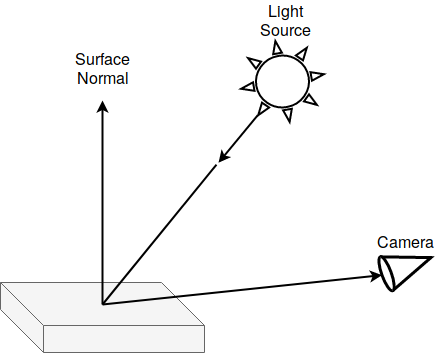
\includegraphics[height=0.2\textheight]{images/surface_normal.png}
	 	\caption{Image configuration for the shape-from-shading problem~\cite{Reflectance_map_techniques}.}
	 	\label{fig:surface_normal}
	\end{figure}
%#########################################################
	\subsection{Orthographic and perspective projection}
	\label{sec:background:projection}
	

%#########################################################
\section{Machine learning usinng CNN}
\label{sec:background:CNN}
- erklären wie CNN funktionieren? 
- Idee für encoder decoder Architektur erklären

%#########################################################
\subsection{Deep Residual Learning}
\label{sec:background:mlCNN:resnet}
	Deep residual neuronal networks 
	In view of the fact that deeper neuronal networks are harder to train
- erklären was ResNet ist \\
- wie funktionieren Residual
- Architektur von ResNet18

	\chapter{Dataset}
\label{sec:dataset}
 	In lack of sufficient training data machine learning approaches to the shape-from-shading problem have been limited. So to fulfill the task of training the MarrNet Architecture 
 	%TODO Marrnet oder CNN 
 	on different perspective projections a new image dataset was necessary. In section \ref{sec:dataset:rendering} is explained, how the Mitsuba renderer~\cite{Mitsuba} is used, to generate the images. 
 	

\section{Shapenet}
\label{sec:dataset:shapenet}
	- warum shape net \\
	- was ist shapene \\
	- wie funktionieren shapenet objekte \\
	- warum die stühle


\section{Rendering}
\label{sec:dataset:rendering}
	- Was ist der Mitsuba renderer, wie funktioniert dieser. \\
	- Welche konfigurationen wurden getroffen um die stühle zu rendern? 
	- Beispiel bilder


%	\begin{figure}
%		\centering
%		\textaccent{\newcommand{\cube}[9]{
	% save values to variables
	\def \CubeHeight {#1}
	\def \CubeWidth {#2}
	\def \CubeDepth {#3}
	\def \CubeX {#4}
	\def \CubeY {#5}
	\def \CubeZ {#6}
	\def \CubeH {#7}
	\def \CubeW {#8}
	\def \CubeL {#9}
	\def \linecolor {black}
	\def \facecolor {\Thesiscolorbright}
	\def \CubeOpacity {0.6}
	
	% define points
	\coordinate (A) at (\CubeX,	       \CubeY,		   \CubeZ+\CubeDepth);
	\coordinate (B) at (\CubeX+\CubeWidth, \CubeY,         \CubeZ+\CubeDepth);
	\coordinate (C) at (\CubeX,        \CubeY+\CubeHeight, \CubeZ+\CubeDepth);
	\coordinate (D) at (\CubeX+\CubeWidth, \CubeY+\CubeHeight, \CubeZ+\CubeDepth);
	\coordinate (E) at (\CubeX,		   \CubeY,		   \CubeZ);
	\coordinate (F) at (\CubeX+\CubeWidth, \CubeY,		   \CubeZ);
	\coordinate (G) at (\CubeX,		   \CubeY+\CubeHeight, \CubeZ);
	\coordinate (H) at (\CubeX+\CubeWidth, \CubeY+\CubeHeight, \CubeZ);
	
	% create surfaces
	\draw[\linecolor,fill=\facecolor,opacity=\CubeOpacity] 
			(A) -- (B) -- (F) -- (E) -- cycle;% Bottom Face
	\draw[\linecolor,fill=\facecolor,opacity=\CubeOpacity] 
			(E) -- (F) -- (H) -- (G) -- cycle;% Back Face
	\draw[\linecolor,fill=\facecolor,opacity=\CubeOpacity] 
			(A) -- (C) -- (G) -- (E) -- cycle;% Left Face
	\draw[\linecolor,fill=\facecolor,opacity=\CubeOpacity] 
			(B) -- (D) -- (H) -- (F) -- cycle;% Right Face
	\draw[\linecolor,fill=\facecolor,opacity=\CubeOpacity] 
			(C) -- (D) -- (H) -- (G) -- cycle;% Top Face
	\draw[\linecolor,fill=\facecolor,opacity=\CubeOpacity] 
	(A) -- (B) -- (D) -- (C) -- cycle;% Front Face
			
	\node [label={below:\tiny{$\CubeH\times \CubeW\times \CubeL$}}] at ( $ (A)!0.5!(B) $ ) (T) {};
	
%	% Following is for debugging purposes to see where the points are
%	% These are last so that they show up on top
%	\foreach \xy in {A, B, C, D, E, F, G, H}{
%	    \node at (\xy) {\tiny{\xy}};
%	}
}

\newcommand{\cubedotted}[9]{
% save values to variables
\def \CubeHeight {#1}
\def \CubeWidth {#2}
\def \CubeDepth {#3}
\def \CubeX {#4}
\def \CubeY {#5}
\def \CubeZ {#6}
\def \CubeH {#7}
\def \CubeW {#8}
\def \CubeL {#9}
\def \linecolor {black}
\def \facecolor {\Thesiscolorbright}
\def \CubeOpacity {0.8}

% define points
\coordinate (A) at (\CubeX,	       \CubeY,		   \CubeZ+\CubeDepth);
\coordinate (B) at (\CubeX+\CubeWidth, \CubeY,         \CubeZ+\CubeDepth);
\coordinate (C) at (\CubeX,        \CubeY+\CubeHeight, \CubeZ+\CubeDepth);
\coordinate (D) at (\CubeX+\CubeWidth, \CubeY+\CubeHeight, \CubeZ+\CubeDepth);
\coordinate (E) at (\CubeX,		   \CubeY,		   \CubeZ);
\coordinate (F) at (\CubeX+\CubeWidth, \CubeY,		   \CubeZ);
\coordinate (G) at (\CubeX,		   \CubeY+\CubeHeight, \CubeZ);
\coordinate (H) at (\CubeX+\CubeWidth, \CubeY+\CubeHeight, \CubeZ);

% create surfaces
\draw[\linecolor,fill=\facecolor,opacity=\CubeOpacity] 
(A) -- (B) -- (F) -- (E) -- cycle;% Bottom Face
\draw[\linecolor,fill=\facecolor,opacity=\CubeOpacity] 
(E) -- (F) -- (H) -- (G) -- cycle;% Back Face
\draw[\linecolor,fill=\facecolor,opacity=\CubeOpacity] 
(A) -- (C) -- (G) -- (E) -- cycle;% Left Face
\draw[\linecolor,fill=\facecolor,opacity=\CubeOpacity] 
(B) -- (D) -- (H) -- (F) -- cycle;% Right Face
\draw[\linecolor,fill=\facecolor,opacity=\CubeOpacity] 
(C) -- (D) -- (H) -- (G) -- cycle;% Top Face
\draw[\linecolor,fill=\facecolor,opacity=\CubeOpacity] 
(A) -- (B) -- (D) -- (C) -- cycle;% Front Face

\node [label={below:\tiny{$\CubeH\times \CubeW\times \CubeL$}}] at ( $ (A)!0.5!(B) $ ) (T) {};
\node [label={left:$z$}] at ( $ (A)!0.5!(G) $ ) {};

\coordinate (BP) at (\CubeX+\CubeWidth+1+0.01cm, \CubeY,         \CubeZ+\CubeDepth);
\coordinate (DP) at (\CubeX+\CubeWidth+1+0.01cm, \CubeY+\CubeHeight, \CubeZ+\CubeDepth);
\coordinate (FP) at (\CubeX+\CubeWidth+1+0.01cm, \CubeY,		   \CubeZ);
\coordinate (HP) at (\CubeX+\CubeWidth+1+0.01cm, \CubeY+\CubeHeight, \CubeZ);
\draw [densely dashed,thick,->] (A) -- (BP);
\draw [densely dashed,thick,->] (C) -- (DP);
\draw [densely dashed,thick,->] (G) -- (HP);
\draw [densely dashed,thick,->] (E) -- (FP);

%	% Following is for debugging purposes to see where the points are
%	% These are last so that they show up on top
%	\foreach \xy in {A, B, C, D, E, F, G, H}{
%	    \node at (\xy) {\tiny{\xy}};
%	}
}

\newcommand{\cubenotext}[6]{
% save values to variables
\def \CubeHeight {#1}
\def \CubeWidth {#2}
\def \CubeDepth {#3}
\def \CubeX {#4}
\def \CubeY {#5}
\def \CubeZ {#6}
\def \linecolor {black}
\def \facecolor {\Thesiscolorbright}
\def \CubeOpacity {0.8}

% define points
\coordinate (A) at (\CubeX,	       \CubeY,		   \CubeZ+\CubeDepth);
\coordinate (B) at (\CubeX+\CubeWidth, \CubeY,         \CubeZ+\CubeDepth);
\coordinate (C) at (\CubeX,        \CubeY+\CubeHeight, \CubeZ+\CubeDepth);
\coordinate (D) at (\CubeX+\CubeWidth, \CubeY+\CubeHeight, \CubeZ+\CubeDepth);
\coordinate (E) at (\CubeX,		   \CubeY,		   \CubeZ);
\coordinate (F) at (\CubeX+\CubeWidth, \CubeY,		   \CubeZ);
\coordinate (G) at (\CubeX,		   \CubeY+\CubeHeight, \CubeZ);
\coordinate (H) at (\CubeX+\CubeWidth, \CubeY+\CubeHeight, \CubeZ);

% create surfaces
\draw[\linecolor,fill=\facecolor] 
(A) -- (B) -- (F) -- (E) -- cycle;% Bottom Face
\draw[\linecolor,fill=\facecolor] 
(E) -- (F) -- (H) -- (G) -- cycle;% Back Face
\draw[\linecolor,fill=\facecolor] 
(A) -- (C) -- (G) -- (E) -- cycle;% Left Face
\draw[\linecolor,fill=\facecolor,opacity=\CubeOpacity] 
(B) -- (D) -- (H) -- (F) -- cycle;% Right Face
\draw[\linecolor,fill=\facecolor,opacity=\CubeOpacity] 
(C) -- (D) -- (H) -- (G) -- cycle;% Top Face
\draw[\linecolor,fill=\facecolor,opacity=\CubeOpacity] 
(A) -- (B) -- (D) -- (C) -- cycle;% Front Face

%	% Following is for debugging purposes to see where the points are
%	% These are last so that they show up on top
%	\foreach \xy in {A, B, C, D, E, F, G, H}{
%	    \node at (\xy) {\tiny{\xy}};
%	}
}

\begin{tikzpicture}[scale=1]
\newcommand{\Boxcolor}{\Thesiscolorbright}
\newcommand{\Linecolor}{black}
\newcommand{\halve}{0.3}

% define values
\pgfmathsetmacro\scale{1/100}
\pgfmathsetmacro\LayerDist{80}
\pgfmathsetmacro\THW{192 * \scale}
\pgfmathsetmacro\THWFactor{0.7}
\pgfmathsetmacro\TFirstLayer{3 * \scale}
\pgfmathsetmacro\TLayer{\TFirstLayer*(5+1/3)}
\pgfmathsetmacro\TLayerFactor{1.5}
\pgfmathsetmacro\XShift{350 * \scale}
\pgfmathsetmacro\YShift{0 * \scale}
\pgfmathsetmacro\ZShift{0 * \scale}

% first network part
\cube{\THW}{\TFirstLayer}{\THW}{\XShift}{\YShift}{\ZShift}{256}{256}{3}

\pgfmathsetmacro\XShiftInc{\TLayer + \LayerDist * \scale}

% add text
\node at ({\XShift+\XShiftInc/2},2.2,0) {\tiny{7x7 conv}};

\pgfmathsetmacro\THW{\THW*\THWFactor}
\pgfmathsetmacro\XShift{\XShift + \TLayer * 0.8 + \LayerDist * \scale}
\pgfmathsetmacro\YShift{\YShift+\THW/4}
\pgfmathsetmacro\ZShift{\ZShift+\THW/4}
\pgfmathsetmacro\TLayer{\TLayer*\TLayerFactor}

\cube{\THW}{\TLayer}{\THW}{\XShift}{\YShift}{\ZShift}{96}{96}{16}
\pgfmathsetmacro\XShiftInc{\TLayer + \LayerDist * \scale}

% add text
\node at ({\XShift+\XShiftInc/2},2.2,0) {\tiny{CONV2}};

\pgfmathsetmacro\THW{\THW*\THWFactor}
\pgfmathsetmacro\XShift{\XShift + \TLayer * 0.8 + \LayerDist * \scale}
\pgfmathsetmacro\YShift{\YShift+\THW/4}
\pgfmathsetmacro\ZShift{\ZShift+\THW/4}
\pgfmathsetmacro\TLayer{\TLayer*\TLayerFactor}

\cube{\THW}{\TLayer}{\THW}{\XShift}{\YShift}{\ZShift}{48}{48}{32}
\pgfmathsetmacro\XShiftInc{\TLayer + \LayerDist * \scale}

% add text
\node at ({\XShift+\XShiftInc/2},2.2,0) {\tiny{CONV3}};

\pgfmathsetmacro\THW{\THW*\THWFactor}
\pgfmathsetmacro\XShift{\XShift + \TLayer * 0.8 + \LayerDist * \scale}
\pgfmathsetmacro\YShift{\YShift+\THW/4}
\pgfmathsetmacro\ZShift{\ZShift+\THW/4}
\pgfmathsetmacro\TLayer{\TLayer*\TLayerFactor}

\cube{\THW}{\TLayer}{\THW}{\XShift}{\YShift}{\ZShift}{24}{24}{64}
\pgfmathsetmacro\XShiftInc{\TLayer + \LayerDist * \scale}

% add text
\node at ({\XShift+\XShiftInc/2},2.2,0) {\tiny{CONV4}};

\pgfmathsetmacro\THW{\THW*\THWFactor}
\pgfmathsetmacro\XShift{\XShift + \TLayer * 0.8 + \LayerDist * \scale}
\pgfmathsetmacro\YShift{\YShift+\THW/4}
\pgfmathsetmacro\ZShift{\ZShift+\THW/4}
\pgfmathsetmacro\TLayer{\TLayer*\TLayerFactor}

\cube{\THW}{\TLayer}{\THW}{\XShift}{\YShift}{\ZShift}{12}{12}{128}
\pgfmathsetmacro\XShiftInc{\TLayer + \LayerDist * \scale}

% add text
\node at ({\XShift+\XShiftInc/2},2.2,0) {\tiny{CONV5}};

\pgfmathsetmacro\THW{\THW*\THWFactor}
\pgfmathsetmacro\XShift{\XShift + \TLayer * 0.8 + \LayerDist * \scale}
\pgfmathsetmacro\YShift{\YShift+\THW/4}
\pgfmathsetmacro\ZShift{\ZShift+\THW/4}
\pgfmathsetmacro\TLayer{\TLayer*\TLayerFactor}

\cube{\THW}{\TLayer}{\THW}{\XShift}{\YShift}{\ZShift}{6}{6}{256}
\pgfmathsetmacro\XShiftInc{\TLayer + \LayerDist * \scale}

% add text
\node at ({\XShift+\XShiftInc/2},2.2,0) {\tiny{CONV6}};

\pgfmathsetmacro\THW{\THW*\THWFactor}
\pgfmathsetmacro\XShift{\XShift + \TLayer * 0.8 + \LayerDist * \scale}
\pgfmathsetmacro\YShift{\YShift+\THW/4}
\pgfmathsetmacro\ZShift{\ZShift+\THW/4}
\pgfmathsetmacro\TLayer{\TLayer*\TLayerFactor}

\cube{\THW}{\TLayer}{\THW}{\XShift}{\YShift}{\ZShift}{3}{3}{512}

% concatenation
\pgfmathsetmacro\XShift{250 * \scale}
\pgfmathsetmacro\YShift{-500 * \scale}
\pgfmathsetmacro\ZShift{0}
\cube{\THW}{\TLayer}{\THW}{\XShift}{\YShift}{\ZShift}{3}{3}{512}
\pgfmathsetmacro\XShift{\XShift + \TLayer + 50 * \scale}
\node at (\XShift,{\YShift+\THW/4},\ZShift) {\huge{$\oplus$}};
\node [label=above:\tiny{CONCAT}] at (\XShift,{\YShift+\THW/4+0.5},\ZShift) {};
\pgfmathsetmacro\XShift{\XShift + 50 * \scale}
\cube{\THW}{\TLayer}{\THW}{\XShift}{\YShift}{\ZShift}{3}{3}{512}
\coordinate (ZTL) at ({\XShift+\TLayer/2-0.1},-2.1);
\coordinate (ZBR) at ({\XShift+\TLayer/2+0.1},-3.1);
\draw [black,fill=\Thesiscolorbright] (ZTL) rectangle (ZBR);
\node [label={right:$z$}] at ( $ (ZTL)!0.5!(ZBR) $ ) {};
\node [label={left:\tiny{100}}] at ( $ (ZTL)!0.5!(ZBR) $ ) {};
\coordinate (ZBC) at ({\XShift+\TLayer/2},{(-2.8+\YShift)/2});
\node at (ZBC) {\huge{$\downarrow$}};
\node[label={right:\tiny{FULLY}}] at (ZBC) {};


% resizing
\node at ({\XShift + \TLayer + (200 * \scale)/2},{\YShift+\THW/4},\ZShift) {\huge{$\rightarrow$}};
\node [label=above:\tiny{RESIZE}] at ({\XShift + \TLayer + (200 * \scale)/2},{\YShift+\THW/4+0.5},\ZShift) {};
\pgfmathsetmacro\XShift{\XShift + \TLayer + 200 * \scale}
\pgfmathsetmacro\TLayer{\TLayer*2}
\pgfmathsetmacro\THW{(\THW * 4 * \THWFactor) / 3}
\cube{\THW}{\TLayer}{\THW}{\XShift}{\YShift}{\ZShift}{4}{4}{1024}


% second network part
\pgfmathsetmacro\XShift{0 * \scale}
\pgfmathsetmacro\YShift{\YShift - 300 * \scale}
\pgfmathsetmacro\ZShift{0}


\cube{\THW}{\TLayer}{\THW}{\XShift}{\YShift}{\ZShift}{4}{4}{1024}

\pgfmathsetmacro\THW{\THW/\THWFactor}
\pgfmathsetmacro\XShift{\XShift + \TLayer * 0.9 + \LayerDist * \scale}
\pgfmathsetmacro\YShift{\YShift-\THW/4}
\pgfmathsetmacro\ZShift{\ZShift-\THW/4}
\pgfmathsetmacro\TLayer{\TLayer/\TLayerFactor}

% add text
\pgfmathsetmacro\XShiftInc{\LayerDist * \scale / 2}
\node[anchor=base] at ({\XShift-\XShiftInc},-7,-0.5) {\tiny{TCONV1}};
\cube{\THW}{\TLayer}{\THW}{\XShift}{\YShift}{\ZShift}{8}{8}{512}

\pgfmathsetmacro\THW{\THW/\THWFactor}
\pgfmathsetmacro\XShift{\XShift + \TLayer * 0.9 + \LayerDist * \scale}
\pgfmathsetmacro\YShift{\YShift-\THW/4}
\pgfmathsetmacro\ZShift{\ZShift-\THW/4}
\pgfmathsetmacro\TLayer{\TLayer/\TLayerFactor}

% add text
\pgfmathsetmacro\XShiftInc{\LayerDist * \scale / 2}
\node[anchor=base] at ({\XShift-\XShiftInc},-7,-0.5) {\tiny{TCONV2}};
\cube{\THW}{\TLayer}{\THW}{\XShift}{\YShift}{\ZShift}{16}{16}{256}

\pgfmathsetmacro\THW{\THW/\THWFactor}
\pgfmathsetmacro\XShift{\XShift + \TLayer * 0.9 + \LayerDist * \scale}
\pgfmathsetmacro\YShift{\YShift-\THW/4}
\pgfmathsetmacro\ZShift{\ZShift-\THW/4}
\pgfmathsetmacro\TLayer{\TLayer/\TLayerFactor}

% add text
\pgfmathsetmacro\XShiftInc{\LayerDist * \scale / 2}
\node[anchor=base] at ({\XShift-\XShiftInc},-7,-0.5) {\tiny{TCONV3}};
\cube{\THW}{\TLayer}{\THW}{\XShift}{\YShift}{\ZShift}{32}{32}{128}

\pgfmathsetmacro\THW{\THW/\THWFactor}
\pgfmathsetmacro\XShift{\XShift + \TLayer * 0.9 + \LayerDist * \scale}
\pgfmathsetmacro\YShift{\YShift-\THW/4}
\pgfmathsetmacro\ZShift{\ZShift-\THW/4}
\pgfmathsetmacro\TLayer{\TLayer/\TLayerFactor}

% add text
\pgfmathsetmacro\XShiftInc{\LayerDist * \scale / 2}
\node[anchor=base] at ({\XShift-\XShiftInc},-7,-0.5) {\tiny{TCONV4}};
\cube{\THW}{\TLayer}{\THW}{\XShift}{\YShift}{\ZShift}{64}{64}{64}

\pgfmathsetmacro\THW{\THW/\THWFactor}
\pgfmathsetmacro\XShift{\XShift + \TLayer * 0.9 + \LayerDist * \scale}
\pgfmathsetmacro\YShift{\YShift-\THW/4}
\pgfmathsetmacro\ZShift{\ZShift-\THW/4}
\pgfmathsetmacro\TLayer{\TLayer/\TLayerFactor}

% add text
\pgfmathsetmacro\XShiftInc{\LayerDist * \scale / 2}
\node[anchor=base] at ({\XShift-\XShiftInc},-7,-0.5) {\tiny{TCONV5}};
\cube{\THW}{\TLayer}{\THW}{\XShift}{\YShift}{\ZShift}{64}{64}{32}

\pgfmathsetmacro\XShift{\XShift + \TLayer * 0.8 + \LayerDist * \scale + 0.5}
\pgfmathsetmacro\TLayer{3 * \scale}
\cube{\THW}{\TLayer}{\THW}{\XShift}{\YShift}{\ZShift}{64}{64}{3}

\pgfmathsetmacro\XShiftInc{\LayerDist * \scale / 2}
\node[anchor=base] at ({\XShift-\XShiftInc},-7,-0.5) {\tiny{TCONV6}};

% arrows
\draw[rounded corners=7pt, ->, thick](13,0.6) -- (14,0.6) -- (14,-1.5) -- (1,-1.5) -- (1,-4.95) -- (2,-4.95);
\draw[rounded corners=7pt, ->, thick](13.3,-4.95) -- (14.3,-4.95) -- (14.3,-6) -- (-1.5,-6) -- (-1.5,-8) -- (-0.5,-8);
\end{tikzpicture}}
%		\caption{Generator Architecture with face replacement by $\genInputZ$}
%		\label{fig:gen:face}
%	\end{figure}

	

%\section{Supervised Loss Functions}
	\chapter{Model}


\section{MarrNet}
\label{sec:model:marrnet}
- was ist die MarrNet \\
- beschreibung der Architektur 

	\chapter{Experiments}
\label{sec:exp}


\section{Training}
\label{sec:exp:train}
- Besonderheiten beim training?

\subsection{Loss Function}	
\label{sec:exp:train:loss}

\section{Tests}
\label{sec:exp:test}
- Ergebnisse alle gegen gleiche perspektiviche verzerrung \\
- Ergebnisse alle gegen anderere Verzerrungen \\
- Train auf allen gegen bestimmte verzerungen 
	

	\chapter{Conclusion}


%\section{Supervised Loss Functions}
	
	% --- List of figures and tables --- %
	\clearpage
	\listoffigures
	\listoftables
	
	% --- Bibliography --- %
	\bibliography{bib/bibliography}{}
	\bibliographystyle{plain}
	
\end{document}
